   
\date{}

\documentclass[12pt]{article}
\thispagestyle{empty}
\usepackage{tikz} 
\usepackage{graphicx}
\usepackage{amsmath}
\begin{document}

\section{Online Kmeans}
Comparing our version of online kmeans and the one in scikit-learn we observe an exponential increase of the resources (memory and time) while the number of samples increase. In the plot our version of means is plotted in green and the scikit-learn in red. The number of samples is represented using logarithm in base 2.\\
In order to improve our version we implemented an exit strategy inspired from the scikit code. In each iteration of the algorithm we evaluate the inertia of the cluster (sum of the distances off all the points from the closer centroid) and we break out of the for loop when there is not any improvement on the inertia for 10 cycles in a row. With this strategy we improve a little the time exponential behaviour (see plots fist and second version).

\begin{table}
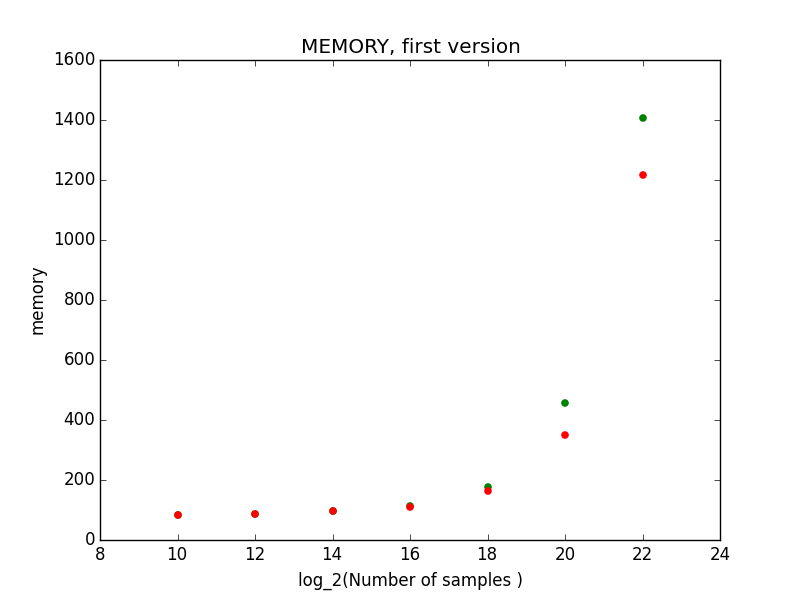
\includegraphics[scale=0.4]{memory_FirstVersion.png}
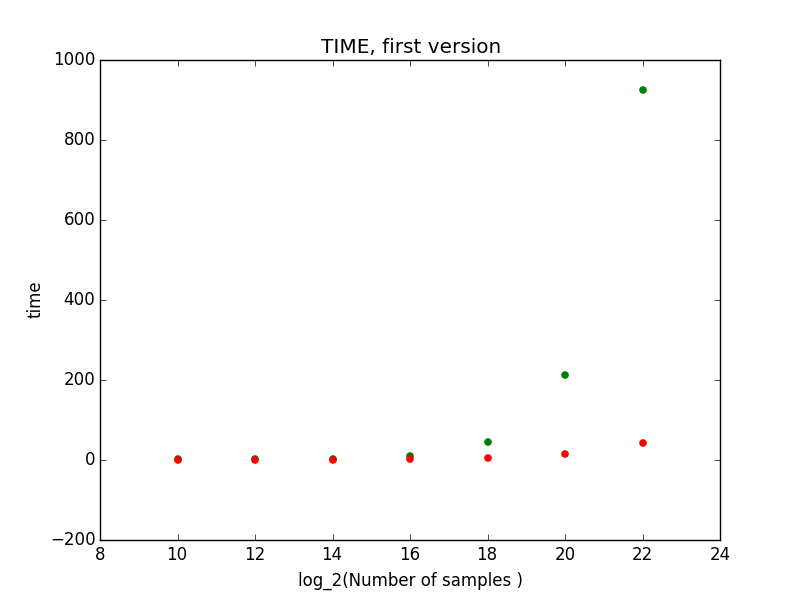
\includegraphics[scale=0.4]{time_FirstVersion.png}
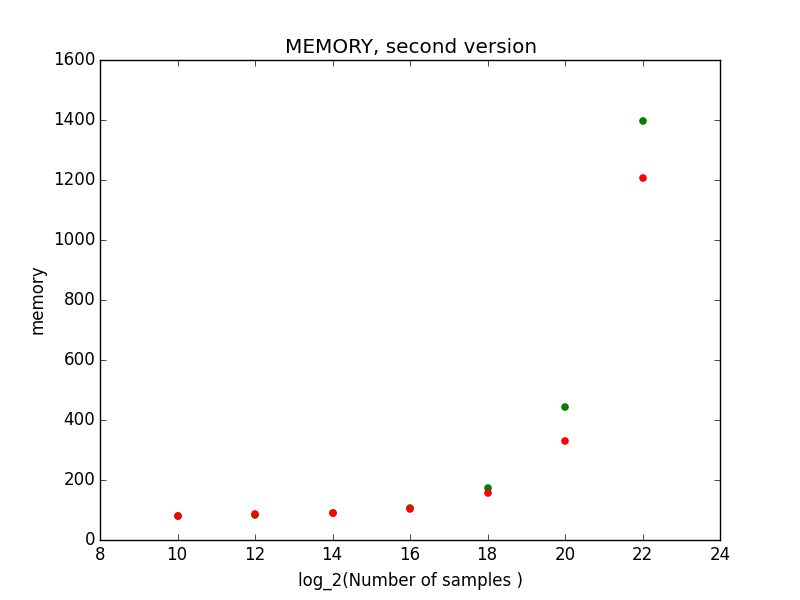
\includegraphics[scale=0.4]{memory_SecondVersion.png}
\includegraphics[scale=0.4]{time_secondVersion.png}
  \end{table}
  
  
  \newpage
\section{Kmeans plus plus}
we have implemented the kmeans++ with the same exit strategy we used for the online kmeans and than compared the two version we had. In the plot, online kmeans (in green) perform better than kmeans++ (in red) for a big number of samples 

  
  
\begin{table}
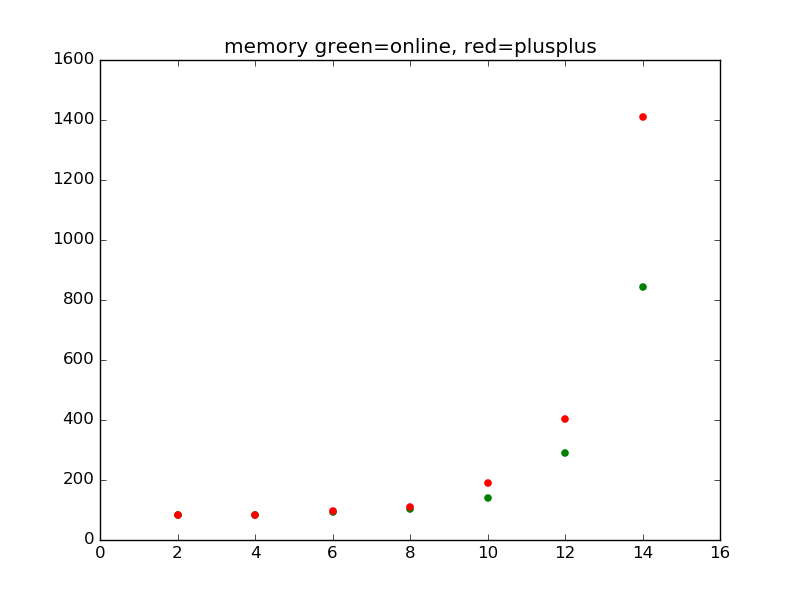
\includegraphics[scale=0.4]{memoryComparison.png}
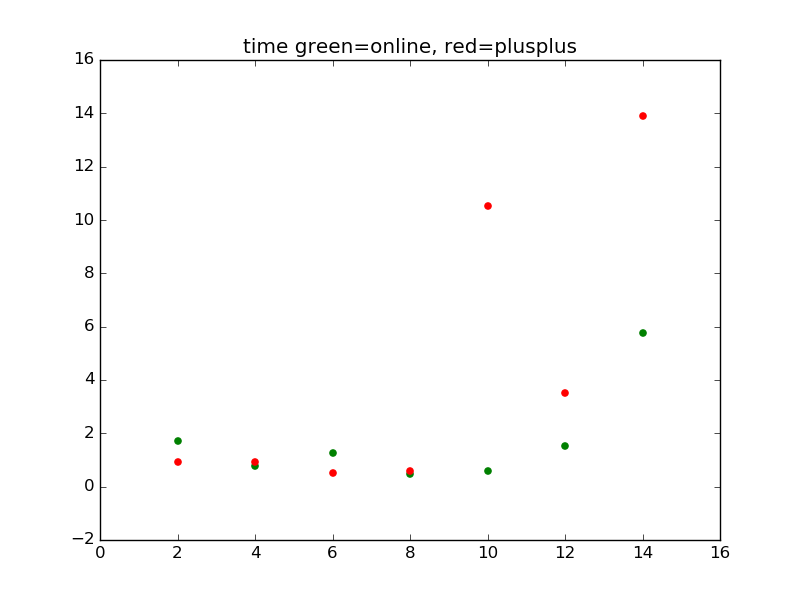
\includegraphics[scale=0.4]{timeComparison.png}
  \end{table}



  \end{document}